\documentclass[11pt,a4paper]{article}
\usepackage[margin=18mm]{geometry}
\usepackage{amsmath,amssymb,booktabs,tikz,enumitem}
\usetikzlibrary{shapes.geometric,positioning,calc}
\setlength{\parindent}{0pt}
\setlength{\parskip}{5pt}
\pagestyle{plain}
\tikzset{ent/.style={draw,rectangle,minimum height=8mm,minimum width=24mm,font=\small},
 weak/.style={ent,path picture={\draw ([xshift=2pt,yshift=2pt]path picture bounding box.south west) rectangle ([xshift=-2pt,yshift=-2pt]path picture bounding box.north east);}},
 rel/.style={draw,diamond,aspect=2,inner sep=2pt,font=\small},
 ident/.style={rel,double,double distance=1.2pt},
 attr/.style={draw,ellipse,inner sep=3pt,font=\small},
 multi/.style={attr,double,double distance=1pt},
 derived/.style={attr,dashed}}
\newcommand{\pk}[1]{\underline{\mathit{#1}}}
\newcommand{\partkey}[1]{\shortstack{#1\\[-5pt]\scriptsize - - - - -}}
\newcommand{\total}[2]{\draw[double,double distance=1.2pt] (#1)--(#2);}
\begin{document}
\begin{center}{\Large\bfseries CSC5041 Assignment 1}\\[3pt]
Concise answers\end{center}
\section*{Question 1 (5 marks)}
\textbf{ER diagram: relationships}
\begin{center}
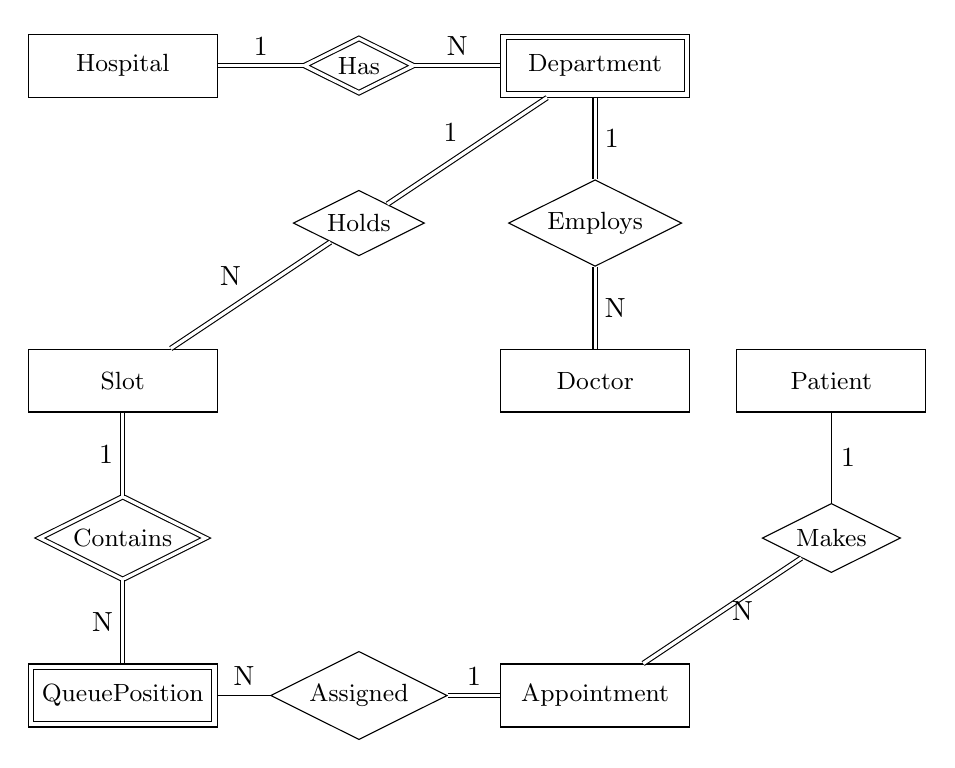
\begin{tikzpicture}[x=1cm,y=1cm]
\node[ent](h) at(0,0){Hospital};
\node[ident](hd) at(3,0){Has};
\node[weak](d) at(6,0){Department};
\node[rel](dd) at(6,-2){Employs};
\node[ent](dr) at(6,-4){Doctor};
\node[rel](ds) at(3,-2){Holds};
\node[ent](s) at(0,-4){Slot};
\node[ident](sq) at(0,-6){Contains};
\node[weak](q) at(0,-8){QueuePosition};
\node[rel](aq) at(3,-8){Assigned};
\node[ent](a) at(6,-8){Appointment};
\node[rel](pa) at(9,-6){Makes};
\node[ent](p) at(9,-4){Patient};
\total{h}{hd}\total{hd}{d}
\path(h)--node[above]{1}(hd);\path(hd)--node[above]{N}(d);
\total{d}{dd}\total{dd}{dr}
\path(d)--node[right]{1}(dd);\path(dd)--node[right]{N}(dr);
\total{d}{ds}\total{ds}{s}
\path(d)--node[above left]{1}(ds);\path(ds)--node[above left]{N}(s);
\total{s}{sq}\total{sq}{q}
\path(s)--node[left]{1}(sq);\path(sq)--node[left]{N}(q);
\draw(q)--node[above]{N}(aq);\total{aq}{a}
\path(aq)--node[above]{1}(a);
\draw(p)--node[right]{1}(pa);\total{pa}{a}
\path(pa)--node[right]{N}(a);
\end{tikzpicture}
\end{center}
Double rectangles/diamonds: weak entities/identifying relationships.\\
Double lines: total participation. Attributes are shown on the next two pages.

\textbf{Assignment constraints}

Let $\operatorname{slot}(q)$ be the slot owning queue position $q$, and
$\operatorname{Assigned}(a,q)$ mean that $q$ is allocated to appointment $a$.
\[
\boxed{\operatorname{Included}(a,s)\iff
 \exists q\,[\operatorname{Assigned}(a,q)\land\operatorname{slot}(q)=s]}
\]
\[
\boxed{\operatorname{Assigned}(a,q_1)\land\operatorname{Assigned}(a,q_2)
 \land\operatorname{slot}(q_1)=\operatorname{slot}(q_2)\Rightarrow q_1=q_2}
\]
Thus each included slot has exactly one allocated position; each position is
allocated to at most one appointment (the $1$ on the Appointment side).

\textbf{Assumptions:} Each appointment contains at least one slot. A slot may have
no appointments. Tags are optional. Duration and totalSlots are stored, as requested:
\[
\mathrm{duration}=\mathrm{endTime}-\mathrm{startTime},\qquad
\mathrm{totalSlots}(a)=|\{s:\operatorname{Included}(a,s)\}|.
\]
Slots start and end on the same date; age is derived from dateOfBirth.

\newpage
\section*{Question 1: attributes (1/2)}
Underlined: key. Dashed underline: partial key. Dashed oval: derived attribute.
\begin{center}
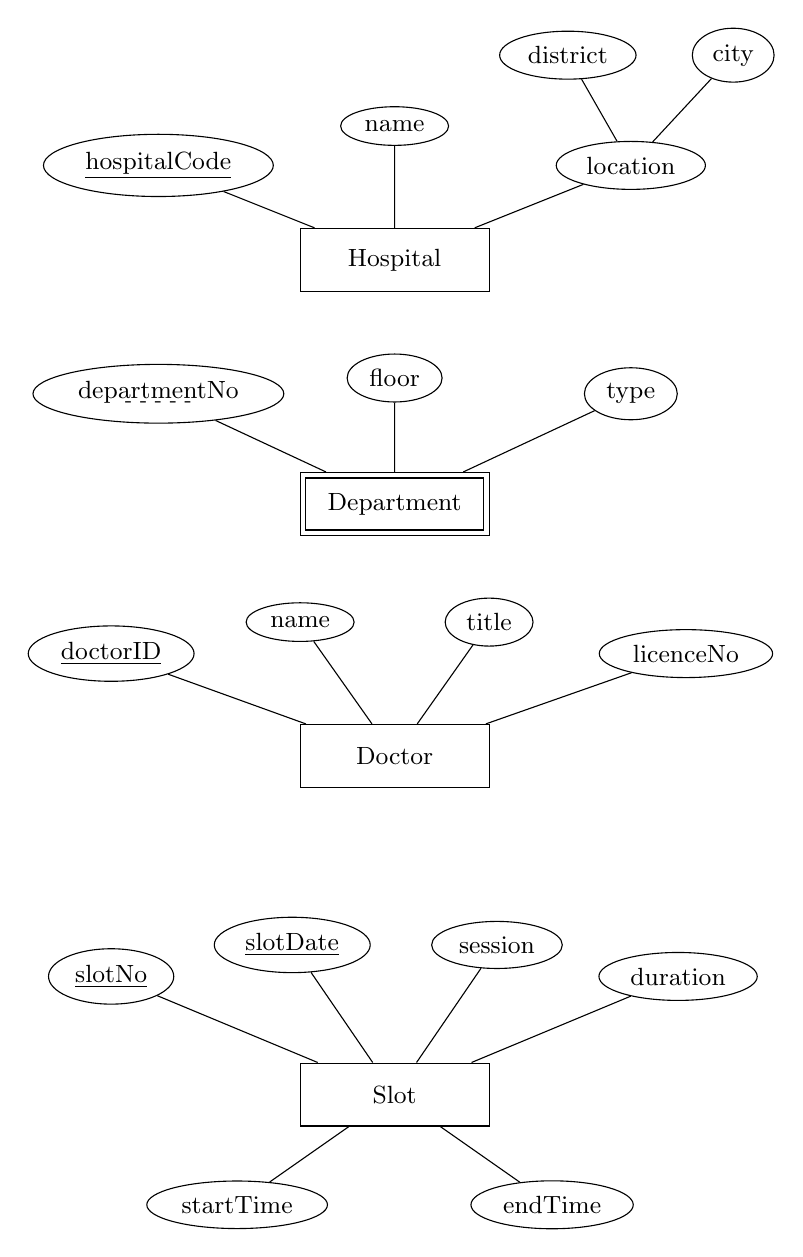
\begin{tikzpicture}[x=1cm,y=1cm]
\node[ent](h) at(0,0){Hospital};
\node[attr](hc) at(-3,1.2){\underline{hospitalCode}};
\node[attr](hn) at(0,1.7){name};
\node[attr](hl) at(3,1.2){location};
\node[attr](hd) at(2.2,2.6){district};\node[attr](hy) at(4.3,2.6){city};
\draw(h)--(hc)(h)--(hn)(h)--(hl)(hl)--(hd)(hl)--(hy);
\node[weak](d) at(0,-3.1){Department};
\node[attr](dn) at(-3,-1.7){\partkey{departmentNo}};
\node[attr](df) at(0,-1.5){floor};\node[attr](dt) at(3,-1.7){type};
\draw(d)--(dn)(d)--(df)(d)--(dt);
\node[ent](dr) at(0,-6.3){Doctor};
\node[attr](di) at(-3.6,-5){\underline{doctorID}};
\node[attr](na) at(-1.2,-4.6){name};\node[attr](ti) at(1.2,-4.6){title};
\node[attr](li) at(3.7,-5){licenceNo};
\draw(dr)--(di)(dr)--(na)(dr)--(ti)(dr)--(li);
\node[ent](s) at(0,-10.6){Slot};
\node[attr](sn) at(-3.6,-9.1){\underline{slotNo}};
\node[attr](sd) at(-1.3,-8.7){\underline{slotDate}};
\node[attr](se) at(1.3,-8.7){session};
\node[attr](du) at(3.6,-9.1){duration};
\node[attr](st) at(-2,-12){startTime};\node[attr](en) at(2,-12){endTime};
\draw(s)--(sn)(s)--(sd)(s)--(se)(s)--(du)(s)--(st)(s)--(en);
\end{tikzpicture}
\end{center}
\[
\begin{aligned}
K_{\rm Hospital}&=(\mathrm{hospitalCode}),\\
K_{\rm Department}&=(\mathrm{hospitalCode},\mathrm{departmentNo}),\\
K_{\rm Doctor}&=(\mathrm{doctorID}),\\
K_{\rm Slot}&=(\mathrm{slotNo},\mathrm{slotDate}).
\end{aligned}
\]
\[
\mathrm{session}\in\{\mathrm{morning},\mathrm{afternoon}\}.
\]
\newpage
\section*{Question 1: attributes (2/2)}
Double oval: multivalued attribute. Repeated entity names denote the same entities.
\begin{center}
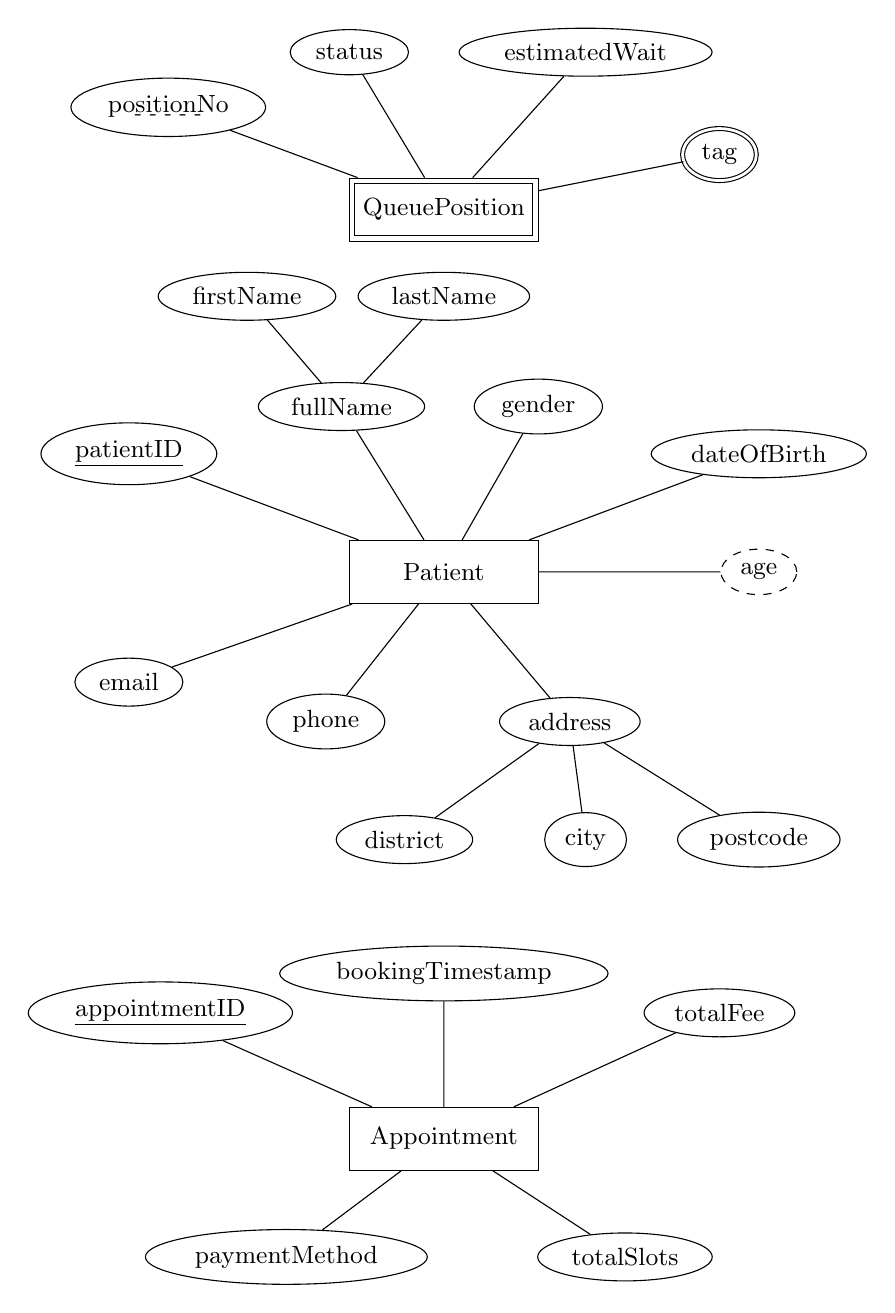
\begin{tikzpicture}[x=1cm,y=1cm]
\node[weak](q) at(0,0){QueuePosition};
\node[attr](qn) at(-3.5,1.3){\partkey{positionNo}};
\node[attr](qs) at(-1.2,2){status};
\node[attr](qw) at(1.8,2){estimatedWait};
\node[multi](qt) at(3.5,.7){tag};
\draw(q)--(qn)(q)--(qs)(q)--(qw)(q)--(qt);
\node[ent](p) at(0,-4.6){Patient};
\node[attr](pi) at(-4,-3.1){\underline{patientID}};
\node[attr](pn) at(-1.3,-2.5){fullName};
\node[attr](pf) at(-2.5,-1.1){firstName};\node[attr](pl) at(0,-1.1){lastName};
\node[attr](pg) at(1.2,-2.5){gender};\node[attr](pb) at(4,-3.1){dateOfBirth};
\node[derived](ag) at(4,-4.6){age};
\node[attr](pe) at(-4,-6){email};\node[attr](pp) at(-1.5,-6.5){phone};
\node[attr](pa) at(1.6,-6.5){address};
\node[attr](pd) at(-.5,-8){district};\node[attr](pc) at(1.8,-8){city};
\node[attr](pz) at(4,-8){postcode};
\draw(p)--(pi)(p)--(pn)(pn)--(pf)(pn)--(pl)(p)--(pg)(p)--(pb)(p)--(ag)
 (p)--(pe)(p)--(pp)(p)--(pa)(pa)--(pd)(pa)--(pc)(pa)--(pz);
\node[ent](a) at(0,-11.8){Appointment};
\node[attr](ai) at(-3.6,-10.2){\underline{appointmentID}};
\node[attr](ab) at(0,-9.7){bookingTimestamp};
\node[attr](af) at(3.5,-10.2){totalFee};
\node[attr](ap) at(-2,-13.3){paymentMethod};\node[attr](at) at(2.3,-13.3){totalSlots};
\draw(a)--(ai)(a)--(ab)(a)--(af)(a)--(ap)(a)--(at);
\end{tikzpicture}
\end{center}
\[
K_{\rm QueuePosition}=(\mathrm{slotNo},\mathrm{slotDate},\mathrm{positionNo}).
\]
estimatedWait is measured in minutes; tag may have zero or more values.
\newpage
\section*{Question 2 (4 marks)}
Underline = primary key. Composite attributes are flattened; multivalued
attributes form a separate relation; derived attributes are omitted.
\[
\boxed{\begin{aligned}
E1&\;(\pk{A1},A2)\\[3pt]
E2&\;(\pk{A9},\pk{A3},A4)\\[3pt]
E3&\;(\pk{A5})\\[3pt]
E3\_A6&\;(\pk{A5},\pk{A6})\\[3pt]
E4&\;(\pk{A7},A8)\\[3pt]
E5&\;(\pk{A9},A12)\\[3pt]
E6&\;(\pk{A12},A14,A15)\\[3pt]
R1&\;(\pk{A1},\pk{A9},\pk{A3},A7)\\[3pt]
R3&\;(\pk{A5},\pk{A12},A16)
\end{aligned}}
\]
\textbf{Foreign keys}
\[
\begin{aligned}
E2.A9&\longrightarrow E5.A9,\\
E3\_A6.A5&\longrightarrow E3.A5,\\
E5.A12&\longrightarrow E6.A12,\\
R1.A1&\longrightarrow E1.A1,\\
R1.(A9,A3)&\longrightarrow E2.(A9,A3),\\
R1.A7&\longrightarrow E4.A7,\\
R3.A5&\longrightarrow E3.A5,\\
R3.A12&\longrightarrow E6.A12.
\end{aligned}
\]
\textbf{Constraints and mapping}
\[
\begin{aligned}
&\operatorname{UNIQUE}(E5.A12),\qquad E5.A12\ne\mathrm{NULL};\\
&\pi_{A1}(R1)=\pi_{A1}(E1),\qquad
 \pi_{A7}(R1)=\pi_{A7}(E4);\\
&\pi_{A12}(R3)=\pi_{A12}(E6).
\end{aligned}
\]
\begin{itemize}[leftmargin=*,itemsep=3pt]
\item $R2$: identifying $1:N$ relationship, absorbed into $E2$ through $A9$.
\item $R4$: $1:1$, with total participation of $E5$; absorbed into $E5$ through $A12$.
\item $R1$: $(A1,A9,A3)\to A7$ (the $1$ on the $E4$ side).
\item $A10,A11$ are derived; $A13$ is replaced by $A14,A15$.
\end{itemize}
\newpage
\section*{Question 3 (6 marks)}
All $\bowtie$ without a condition are natural joins.
Aggregation: $\gamma_{G;\,\mathrm{FUNC}(A)}$ groups by $G$.

\subsection*{1) Car trips in June 2025}
\[
\boxed{\pi_{\mathrm{riderName}}\!\left(
\mathrm{Rider}\bowtie
\sigma_{\substack{\mathrm{category}='car'\,\land\\
\mathrm{tripDate}\ge '2025\text{-}06\text{-}01'\,\land\\
\mathrm{tripDate}< '2025\text{-}07\text{-}01'}}
(\mathrm{Trip}\bowtie\mathrm{VehicleType})\right)}
\]
\subsection*{2) Maximum payment: only trips with fare $\le 10$}
\begin{align*}
G&\leftarrow\pi_{\mathrm{riderID}}(\mathrm{Trip})
 -\pi_{\mathrm{riderID}}(\sigma_{\mathrm{fare}>10}(\mathrm{Trip})),\\[3pt]
\boxed{\mathrm{Answer}}&\boxed{\leftarrow
\gamma_{\mathrm{riderID};\,\mathrm{MAX}(\mathrm{amount})}(G\bowtie\mathrm{Payment})}.
\end{align*}
Here ``has made only trips'' requires at least one trip; MAX is returned for riders
with recorded payments.

\subsection*{3) Riders using every available category}
\begin{align*}
C&\leftarrow\pi_{\mathrm{category}}(\mathrm{VehicleType}),\\
U&\leftarrow\pi_{\mathrm{riderID},\mathrm{category}}
 (\mathrm{Trip}\bowtie\mathrm{VehicleType}),\\
G&\leftarrow U\div C,\\[3pt]
\boxed{\mathrm{Answer}}&\boxed{\leftarrow
\pi_{\mathrm{riderID},\mathrm{membershipTier}}(\mathrm{Rider}\bowtie G)}.
\end{align*}
Assume the system has at least one vehicle category. Retain riderID to identify each rider.

\subsection*{4) Average age, counting every qualifying trip}
\begin{align*}
S&\leftarrow\rho_{(\mathrm{startStationID},\mathrm{zoneID},\mathrm{capacity},\mathrm{stationType})}
 (\mathrm{Station}),\\
T&\leftarrow\sigma_{\substack{\mathrm{zoneName}='Xuhui'\,\land\\
\mathrm{tripDate}\ge '2025\text{-}10\text{-}01'\,\land\\
\mathrm{tripDate}\le '2025\text{-}11\text{-}02'}}
 (\mathrm{Trip}\bowtie S\bowtie\mathrm{Zone}\bowtie\mathrm{Rider}),\\
V&\leftarrow\pi_{\mathrm{tripID},\mathrm{age}}(T),\\[3pt]
\boxed{\mathrm{Answer}}&\boxed{\leftarrow\gamma_{\mathrm{AVG}(\mathrm{age})}(V)}.
\end{align*}
Retaining tripID gives one tuple per trip, even when ages are equal.
\end{document}
